\chapter{Reinforcement Learning Setup}
\label{chapter:RL}
This chapter provides an overview of the process of developing the reinforcement learning (RL) agent that will be used in the development phase of the RL-MPC algorithm. This chapter focuses on the description of the environment on which the RL agent is trained, as well as the performance of the agent in both deterministic and stochastic environments. Finally, the training of a value function for a fixed policy is also investigated. 

\section{Environment Description} \label{section:env-description}
This section describes the environment for the RL agent to learn an optimal policy. The environment is built on the Greenhouse model as described in \autoref{section:greenhouse-model} and outlines important features to successfully train an RL agent. This includes the observation space available for the agent to make decisions on, the action space available to the agent, the reward function, and finally the weather data that is used for the training period.

\paragraph{Observation Space}
The observation space of the agent must be carefully selected, in order to achieve desirable results. Providing too little information may degrade performance; however, giving the agent too much information about the state of the environment may introduce unwanted noise, making it difficult to infer an optimal policy. Typically, the state of dry weight of the lettuce crop would not be available for an expert grower to make decisions on as it is difficult to measure without disrupting the crop's life cycle. However, various methods exist for predicting the state of the crop dry mass such as a non-linear kalman observer \textbf{refXX}. It is assumed the dry mass may be measured and is available to the agent. Other states of the greenhouse, such as the temperature, C02 and humidity levels are easily measured and form part of the observation space. The current weather conditions are also made available to the agent in order to make better decisions. As shown in \textbf{some section}, since the control input is dependent on the previous control input (i.e., it may only deviate a maximum of 10\% from the previous input), it is important to provide the previous control action to the agent. Lastly, the agent is considered to be time-aware, and so the current time step is also given to the agent. Although not necessary, it enables the agent to learn a non-stationary policy. Considering that the growing period is 40 days \textbf{as in Section XXX}, the problem is episodic. By incorporating time awareness, the agent is able to leverage the current time in order to make more optimal decisions. As discussed in \autoref{ssection:optimization-goal} and later in \autoref{paragraph:reward-function}, the optimization goal includes maximizing the growth difference between time steps, and so knowledge of the previous dry mass state, the the growth experienced in the previous time step may be beneficial to learning an optimal policy.
As a result, the 3 following environment state tuples $s(k)$ at time $k$ are separately tested to represent the observation returned to the agent:
\begin{equation}
\label{eq:obs-tuple-1}
    s(k) = (y_1(k),y_2(k),y_3(k),y_4(k), u(k-1), k, d(k))
\end{equation}
\begin{equation}
\label{eq:obs-tuple-2}
\begin{aligned}
    & s(k) = (\Delta y_1(k),y_2(k),y_3(k),y_4(k), u(k-1), k, d(k)) \\
    & \Delta y_1(k) = y_1(k) - y_1(k-1)
\end{aligned}
\end{equation}
\label{eq:obs-tuple-3}
\begin{equation}
    s(k) = (y_1(k-1),y_1(k),y_2(k),y_3(k),y_4(k), u(k-1), k, d(k))
\end{equation}
It is noted, that \autoref{eq:obs-tuple-3} is expected to perform better than \autoref{eq:obs-tuple-1} and \autoref{eq:obs-tuple-2} since more information is provided regarding the Markov decision processes of the model and the reward received, thereby allowing the agent to potential infer the system dynamics more accurately. However \autoref{eq:obs-tuple-1} and \autoref{eq:obs-tuple-2} are simpler, with \autoref{eq:obs-tuple-1} facilitating the learning of a value function and integration in the RL-MPC algorithm as discussed in \textbf{section XXX}. 

\paragraph{Action Space}
The continuous action space, denoted as $A$, is defined as $ \subseteq [-1,1]^3$, where $a \in A$. In order to ensure that the current control input, $u(k)$ satisfies the constraints outlined in  \textbf{show equation}, the agent's action, denoted as $a(k)$, is regarded as a modification to the control input. Consequently, the current control input can be determined as follows:
$$
u(k) = clip(u(k-1) + a(k) \cdot \delta u(k)^{max},u_{min}, u_{max})
$$

where $\delta u(k)^{max},u_{min}, u_{max}$ are defined in \textbf{section here}

\paragraph{Initial Conditions}
Initial conditions were kept constant for every episode for both the stochastic and deterministic case and shown in \autoref{eq:init-conditions}.The values in question were obtained from the sources as cited in \textbf{ref XXX and ref XXX}.

\begin{equation}
    \label{eq:init-conditions}
    \begin{aligned}
        &x(0) = \begin{bmatrix}
            0 & 0 & 0 & 0
        \end{bmatrix}^T \\
        &y(0) = g(x(0)) \\
        &u(0) = \begin{bmatrix}
            0 & 0 & 50
        \end{bmatrix}^T
    \end{aligned}
\end{equation}

\paragraph{Reward Function}
\label{paragraph:reward-function}
The reward function is modelled after the optimization goal as defined in \textbf{section/equation} and represents the same optimization goal as defined for the Model predictive control OCP. Although the van Henten model sufficiently describes the dynamics of lettuce growth in a climate-controlled environment, it does not do so over the entire state space. Therefore state constraints are imposed to ensure states are operated within reasonable limits to ensure realistic conditions. As stated in \textbf{Section XXX}, state constraints cannot be directly imposed but can be indirectly incorporated through a penalty function within the reward function. It is common practice to impose a linear penalty function for state violations when learning a policy with RL for stability reasons \textbf{ref XXX}. As such, the resulting reward function becomes:

\begin{equation}\label{eq:reward_fn}
    \begin{aligned}
        & R(k)  = \kappa_{1} \cdot (y(k)- y(k-1)) - (\kappa_{2} \cdot u_1(k) + \kappa_{3} \cdot u_2(k) + \kappa_{4} \cdot u_3(k))  \\ 
        & - (P_{c02} \cdot y_2(k) + P_T \cdot y_3(k) + P_H \cdot y_4(k))
    \end{aligned}
\end{equation}

where $\kappa_{let},\kappa_{c02},\kappa_{u_v},\kappa_{u_q}$ are defined in \textbf{section XXX} and correspond to the pricing of the the lettuce and control inputs
and the penalty terms $P_{c02},P_T,P_H$ are defined as follows:

\begin{equation}
\begin{aligned}
& P_{\text{CO2}} = 
\begin{cases} 
c_{p_{\text{CO2}}} \cdot (y_2(k) - y_2^{\text{max}}) & \text{if } y_2(k) > y_2^{\text{max}} , \\
c_{p_{\text{CO2}}} \cdot (y_2^{\text{min}} - y_2(k)) & \text{if } y_2(k) < y_2^{\text{min}} , \\
0 & \text{otherwise}
\end{cases}
\\
& P_{T} = 
\begin{cases} 
c_{p_{T_ub}} \cdot (y_3(k) - y_3^{\text{max}}) & \text{if } y_3(k) > y_3^{\text{max}} , \\
c_{p_{T_lb}} \cdot (y_3^{\text{min}} - y_3(k)) & \text{if } y_3(k) < y_3^{\text{min}} , \\
0 & \text{otherwise}
\end{cases}
\\
& P_{H} = 
\begin{cases} 
c_{p_{H}} \cdot (y_4(k) - y_4^{\text{max}}) & \text{if } y_4(k) > y_4^{\text{max}} , \\
c_{p_{H}} \cdot (y_4^{\text{min}} - y_4(k)) & \text{if } y_4(k) < y_4^{\text{min}} , \\
0 & \text{otherwise}
\end{cases}
\\
\end{aligned}
\end{equation}
The penalty constants $c_{p_{\text{CO2}}},c_{p_{T_ub}},c_{p_{T_lb}},c_{p_{H}}$ were found in empirically in \textbf{ref XXX} in order to effectively account for deviations from desired states and their impact on the economic benefit. It should be noted that the upper bound of the temperature  imposes stricter penalties for violations compared to the lower bounds due to the absence of active cooling in the system.  Thus, during periods of increased temperature throughout the day, it is important for the agent to make appropriate decisions. The penalty constants and their respective units are displayed in \autoref{tab:pen-constants}. The selection of minimum and maximum temperatures was based on the typical operating ranges for lettuce crops and the acceptable levels of CO2 for human brief operation.

\begin{table}[h]
    \centering
    \begin{tabular}{|c|c|c|}
    \hline
         parameter& value & units  \\
    \hline
        $c_{p_{\text{CO2}}}$ &$\frac{10^{-3}}{20}$ & \euro$\cdot (ppm \cdot m^2)^{-1}$ \\
        $c_{p_{T_ub}}$ & $\frac{1}{200}$& \euro$\cdot (C^{\circ} \cdot m^2)^{-1}$\\
        $c_{p_{T_lb}}$ & $\frac{1}{300}$& \euro$\cdot (C^{\circ} \cdot m^2)^{-1}$\\
        $c_{p_{H}}$ & $\frac{1}{50}$ & \euro$\cdot (RH_{\%} \cdot m^2)^{-1}$\\
        $y_2^{max}$ & $1600$ & $ppm$ \\
        $y_2^{min}$ & $500$ & $ppm$ \\
        $y_3^{max}$ & $20$ & $C^{\circ}$ \\
        $y_3^{min}$ & $10$ & $C^{\circ}$ \\
        $y_4^{max}$ & $100$ & $RH_{\%}$ \\
        $y_4^{min}$ & $0$ & $RH_{\%}$ \\       
        \hline
    \end{tabular}
    \caption{Penalty Constants}
    \label{tab:pen-constants}
\end{table}
\paragraph{Uncertainty} It is not the focus of this thesis to accurately model the uncertainty in a greenhouse crop environment, however, it is desirable to see the effect of uncertainty on the generated policy for each of the different algorithms. There are several sources of uncertainty in a greenhouse environment, including parametric uncertainty in the model, unmodeled dynamics, measurement uncertainty, and uncertainty in weather forecasts. The various instances of uncertainty observed in different aspects of the environment can ultimately be attributed to the uncertainty that manifests in the system's outputs. Thus, it was determined that in the stochastic case, there exists uncertainty in the change in the states between consecutive time steps. More specifically,for the discrete time model, it may be modelled as:

\begin{equation}
    \label{eq:uncertainty_model}
    \begin{aligned}
     x(k+1) = x(k) + (f(x(k),u(k),d(k) - x(k)) \cdot (1+W),\quad W \sim U(-\sigma, \sigma)  
    \end{aligned}
\end{equation}

where $\sigma$ represents the degree of uncertainty in the evolving states, expressed as a percentage. The uniform distribution was chosen for its higher level of aggressiveness compared to the normal distribution. While it may not accurately represent the uncertainty at hand, it is a useful tool for evaluating the potential variability and risks associated with the various policies generated.



\section{Experimental Setup} \label{section:experimental-setup}

The duration of the growing period for lettuce was determined based on the findings of \textbf{reference XXX}, which indicate that the growing period typically falls within the range of 30 to 50 days. Therefore, a fixed growing period of fixed 40 day was selected. \textbf{Ref XXX} states that discretizing the van Henten model using a time-step between 15 minutes and 1 hour is recommended. Therefore, a time interval of 30 minutes was selected for the purpose of this study. As a result, over a duration of 40 days (1 episode or 1 complete simulation), there is a total of:
$$
k_{total} = \frac{40 \frac{days}{growing \, period} \cdot 24 \frac{hrs}{day} \cdot 60 \frac{min}{hr}}{30 \frac{min}{timestep}} = 1920 \frac{time \, steps}{growing \, period}
$$
The initial interval of 30 minutes was originally set at 15 minutes. However, this decision was revised due to the excessive computational burden it imposed on the MPC solver, with minimal benefits. Consequently, extending the time step enables an exponential speedup in the simulation of the 40-day period, while causing only minor deterioration in performance. As a consequence of this, there is a noticeable increase in the rate at which RL training occurs, thereby allowing for a larger quantity of training episodes.
\\
To facilitate the learning process of RL, the observations returned from the environment were normalized by a running mean and variance. The VecNormalizeWrapper in Stable-Baselines3 is responsible for updating the mean and variance for every observation received from the environment. The observation is normalized as per \autoref{eq:state-normalization} and clipped between $[-10,10]$.

\begin{equation}\label{eq:state-normalization}
    obs_{norm} = \frac{(obs - \mu_{obs}) }{\sqrt{\sigma^2_{obs} + 1\cdot 10^{-8}}}
\end{equation}

where $\mu_{obs}$ and $\sigma^2_{obs}$ represent the running mean and variance, respectively.The value $1\cdot 10^{-8}$ is included to prevent division by zero. Although the VecNormalizeWrapper also facilitates this process, it is necessary to replicate this step when incorporating it into the RL-MPC algorithm. Finally, in order to ensure reproducibility, a seed value of 4 was used for the generation of random numbers.
This seed value was utilized for both the initialization of neural network weights and the selection of actions for exploration purposes.



\paragraph{Weather Data}

\begin{figure}[h]
    \centering
    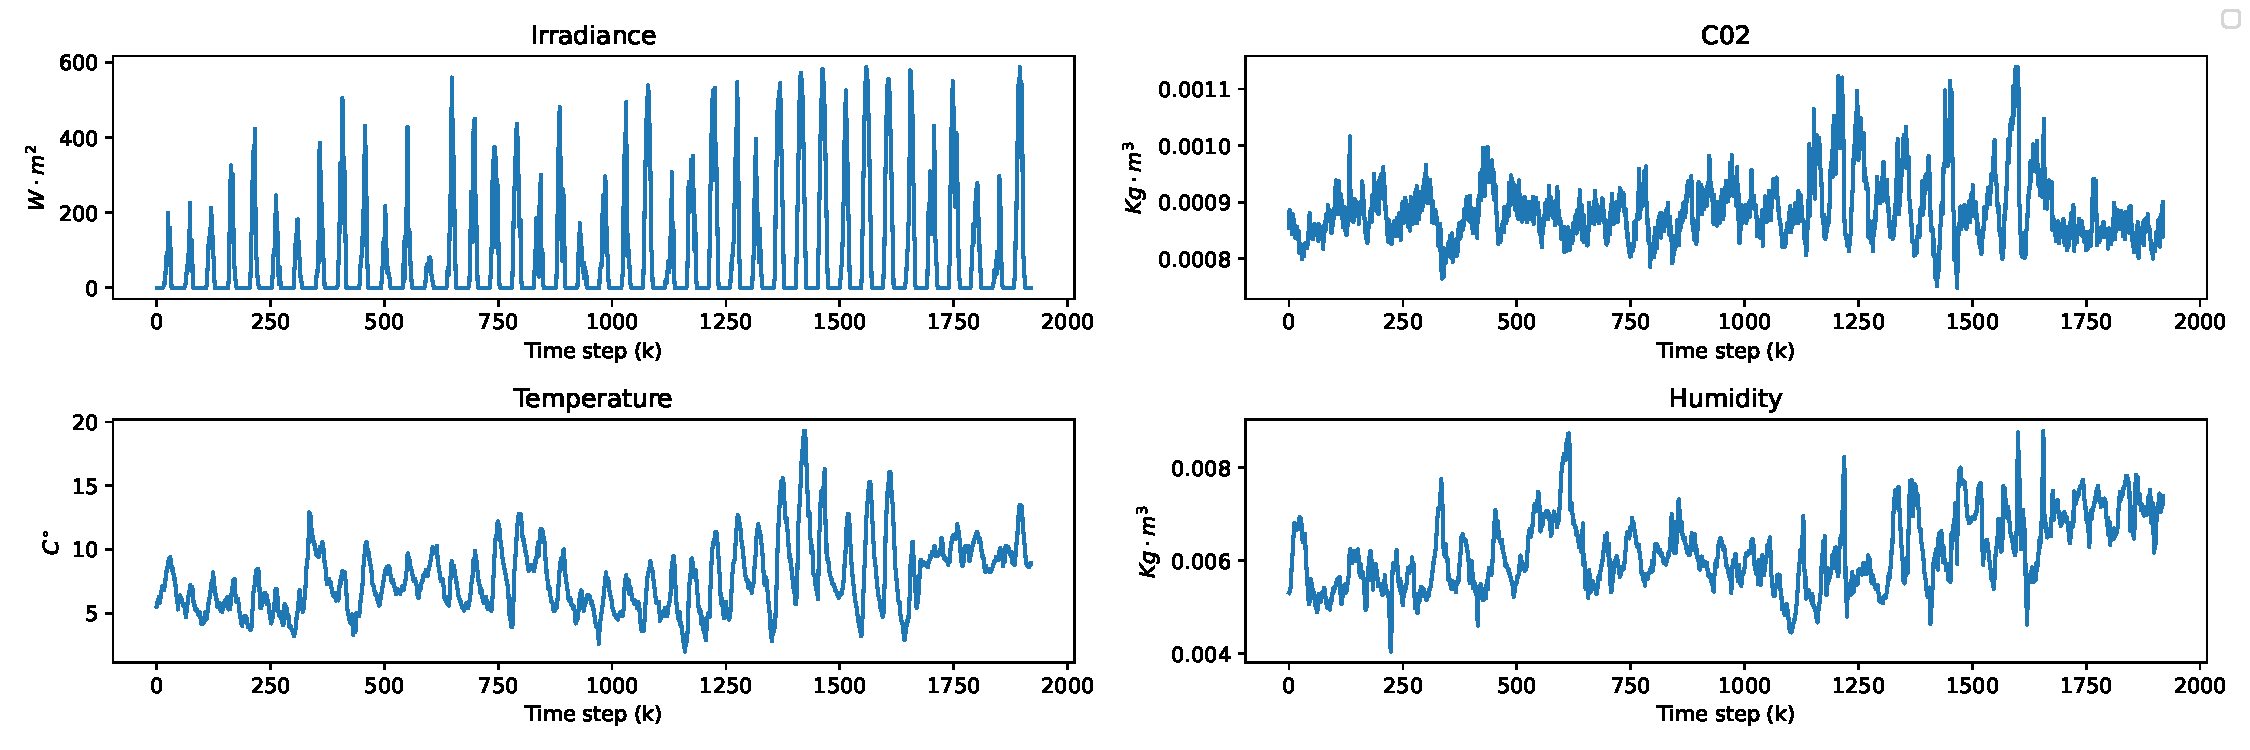
\includegraphics[width=\textwidth]{figures/weather_data.eps}
    \caption{Weather Data}
    \label{fig:weather-data}
\end{figure}

The weather data used in training is obtained from the VenLow Greenhouse in Bleiswijk from the period January 30–March 11, 2014. The weather data was resampled from its original 5-minute interval to a 30-minute interval, in accordance with the timestep of the environment.The weather data remains consistent throughout the episodes, irrespective of whether the training and/or evaluation is conducted under deterministic or stochastic conditions. As such, the validation data is the same as the training data. In practice, it may be necessary to evaluate the agent on unseen weather data, but the thesis aims to develop an RL policy for incorporation with MPC to investigate the resulting controller. Thus, provided that all algorithms/controllers utilize identical weather data, if the agent learns a suitable policy for this specific weather pattern, it can be considered a suitable basis for comparing algorithms.


\paragraph{Deterministic and Stochastic Case}
When learning a policy in both stochastic and deterministic environments, the key distinction lies in the evolution of the state of the greenhouse. In the stochastic case, this evolution follows the principles outlined in \autoref{eq:uncertainty_model}. In the stochastic case, three levels of uncertainty were tested, namely $\sigma = 20\%$,$\sigma = 40\%$ and $\sigma = 80\%$. Although these uncertainty levels might be considered extreme, it was desirable to learn a policy for each of these uncertainty levels to compare to MPC and RL-MPC under identical conditions of uncertainty. The optimal configuration(s) that produce the most favorable outcomes in the deterministic scenario will be employed in the stochastic scenario, and there will be no reevaluation of hyperparameters. WWhile the stochastic environment provides a representation of a scenario closer to real-life conditions, the deterministic case offers a nominal measure of the RL agent's performance and the resulting RL-MPC algorithm when combined with MPC.

\paragraph{Performance Metrics}
The primary performance metric used for evaluating RL agents is the cumulative reward obtained over the 40-day growing period. As demonstrated in \autoref{eq:reward_fn}. The performance metric under consideration is conceptually equivalent to the EPI (\textbf{eq XXX}) minus the summed temperature, C02 and humidity violations. This is a natural selection of the final performance metric as it directly corresponds to what the agent is optimizing, and subsequently, what the MPC and RL-MPC controllers are optimizing. Other metrics include the EPI, total growth, total C02 usage, total heating, computational time to compute control input, temperature and c02 violations. It is difficult to compare these lesser performance metric across policies, since these are all form part of the reward function (with the exception of the computational time) and are not directly optimized. Therefore, making comparisons would not be meaningful, and only observations can be made. However, the computational time taken to compute the optimal control action is an important metric, particularly when combining RL with MPC. 

\section{Hyper-parameter Tuning}
The process of hyper-parameter tuning is frequently laborious and requires exhaustive exploration to determine the best configuration to maximize the cumulative reward of the agent. Therefore, the final hyper-parameters are posted in \autoref{tab:hyper-params} and were found empirically. Refer to \textbf{appendix A} for a more comprehensive analysis of the obtained hyper-parameters. The discount factor and activation function are not reported here. The effect of these two hyper-parameters are important to consider when integrating the value function of the learned agent with MPC. The defaults provided by SB3 are used for hyper-parameters that are not reported.

\begin{table}[h]
    \centering
    \begin{tabular}{|c|c|}
    \hline
        Training Episodes & $100$  \\
        Warm-up episodes &  $9$\\
        Hidden Layers & $2$ \\
        Neurons per Hidden Layer& $128$ \\
        Batch size & $1024$ \\
        Learning Rate & $5\cdot 10^{-3}$ \\
        Buffer size & 100000 \\
        \hline
        
    \end{tabular}
    \caption{Hyper-parameters}
    \label{tab:hyper-params}
\end{table}

\paragraph{Activation Function} The importance of the activation function lies in whether the resulting activation allows the output of the neural network to be differentiable with respect to the inputs. For instance, the ReLu activation function is a commonly used activation function due to its simplicity and superior convergence \textbf{ref XX}. Although ReLu is differentiable with respect to the weight of the neural network, it is not differentiable with respect to the inputs of the neural network. This is important to note since it is necessary for the trained value function to be differentiable with respect to its inputs if it is to be used as a cost function in the MPC formulation. Hence, the tanh function may be used instead, as it is a frequently used activation function that is differentiable with respect to the inputs.

\paragraph{Discount Factor} Another consideration is the discount factor, denoted as $\gamma$. Since the problem is episodic and therefore the cumulative rewards are bounded, it is possible to have a $\gamma = 1$. By setting the discount factor $\gamma$ to 1, the agent is able to consider the entire prediction horizon when making decisions regarding its actions. Additionally, the value function obtained during training satisfies \textbf{equation XXX} indicating that it contains information pertaining to the entire prediction horizon. Having $\gamma < 1$ will shorten the agent's 'prediction horizon' and the resulting value function may not provide significant benefits for the MPC. However, it may stabilize the learning and therefore yield a better policy as compared to when $\gamma = 1$. \\
Results pertaining to the activation function and discount factor are shown and discussed in \autoref{section:rl-deterministic-results}





\section{Deterministic Results}
The outcomes of modifying the discount factor, the activation function, and the impact of the three distinct observations provided to the agent (\autoref{eq:obs-tuple-1}, \autoref{eq:obs-tuple-2}, \autoref{eq:obs-tuple-3}) are presented and examined in this section.Finally, a discussion of the chosen policies and the identification of the desirable characteristics that can be integrated with the MPC framework. While there are several hyperparameters that can impact the performance of the resulting RL policy, this section will focus on the discount factor and activation function. These two hyperparameters are considered necessary aspects of the RL policy, particularly when it is desired to integrate it MPC.


\subsection{Discount Factor}
The tests conducted involved returning the observation to the agent as specified in Equation (2) of the observation tuple, with the hyper parameters as specified in \autoref{tab:hyper-params}. The impact of the discount factor on the agent's performance and the generated value function is investigated. 

\begin{figure}
     \centering
     \begin{subfigure}[b]{0.49\textwidth}
         \centering
         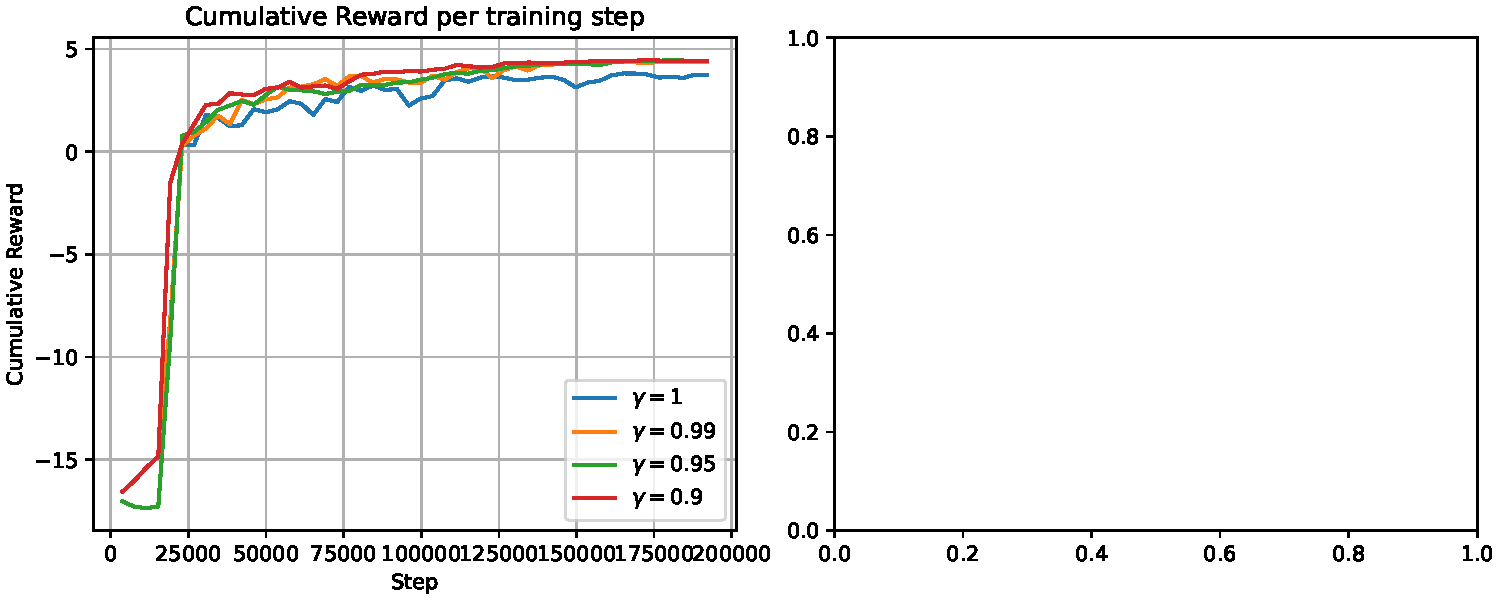
\includegraphics[width=\textwidth]{figures/gamma_reward_training.eps}
         \caption{Cumulative Reward per Training Step}
         \label{fig:gamma_reward_training}
     \end{subfigure}
     \begin{subfigure}[b]{0.49\textwidth}
         \centering
         \includegraphics[width=\textwidth]{figures/gamma_reward_final.eps}
         \caption{Final Cumulative Reward}
         \label{fig:gamma_reward_final}
     \end{subfigure}
        \caption{Discount Factor vs Cumulative Rewards}
        \label{fig:gamma-vs-rewards}
\end{figure}

\paragraph{Performance} 
The cumulative reward achieved over the training period and the final cumulative reward achieved for each different discount factor are depicted in \autoref{fig:gamma_reward_training} and \autoref{fig:gamma_reward_final} respectively.
As can be seen in \autoref{fig:gamma-vs-rewards}, it is clear that $\gamma = 1$ does not perform as well as lower discount factors. It is noted that the degradation in performance comes from the increase in problem complexity when the discount factor is 1. Hence, it becomes more difficult in finding an optimal policy, requiring a different set of hyper-parameters and potentially a significantly larger number of training episodes. However, the policy generated with this discount factor will provide a value function that holds information across the entire time horizon, which is desirable. \\
In the deterministic case, one can assess the accuracy of the obtained value function by comparing the predicted values of each state and time step visited during the 40-day simulation with the actual values of the visited states. In addition, the predicted value of each state may also be compared to the cumulative rewards obtained at each state. One can determine the precise value of each state visited in the simulation by adding up the rewards from that state onwards, as per \textbf{eq XXX}, with the respective discount factor used.

\paragraph{Value Function Approximation}
It is difficult to determine whether the critic has converged. Given that the critic serves as a q-value function approximator, the actor must identify the optimal action for a given state in order to compute the value of that state using the critic. Therefore, convergence of the value function is dependent upon the actor policy as well. Although the training curves indicate that the critic has converged, it has only converged in alignment with the actor. In order to assess whether the critic (and actor) has achieved convergence in predicting the value function, it is possible to visualize and compare the actual and predicted value of a given state.\\
For each discount factor, the predicted value of each state and the cumulative rewards obtained thus far were plotted and evaluated, for the entire 40 day period. It is noted that for the deterministic case, the realizations of state trajectories and rewards received do not differ between simulations, hence the exact value of each state may be calculated. 


\begin{figure}[H]
    \centering
    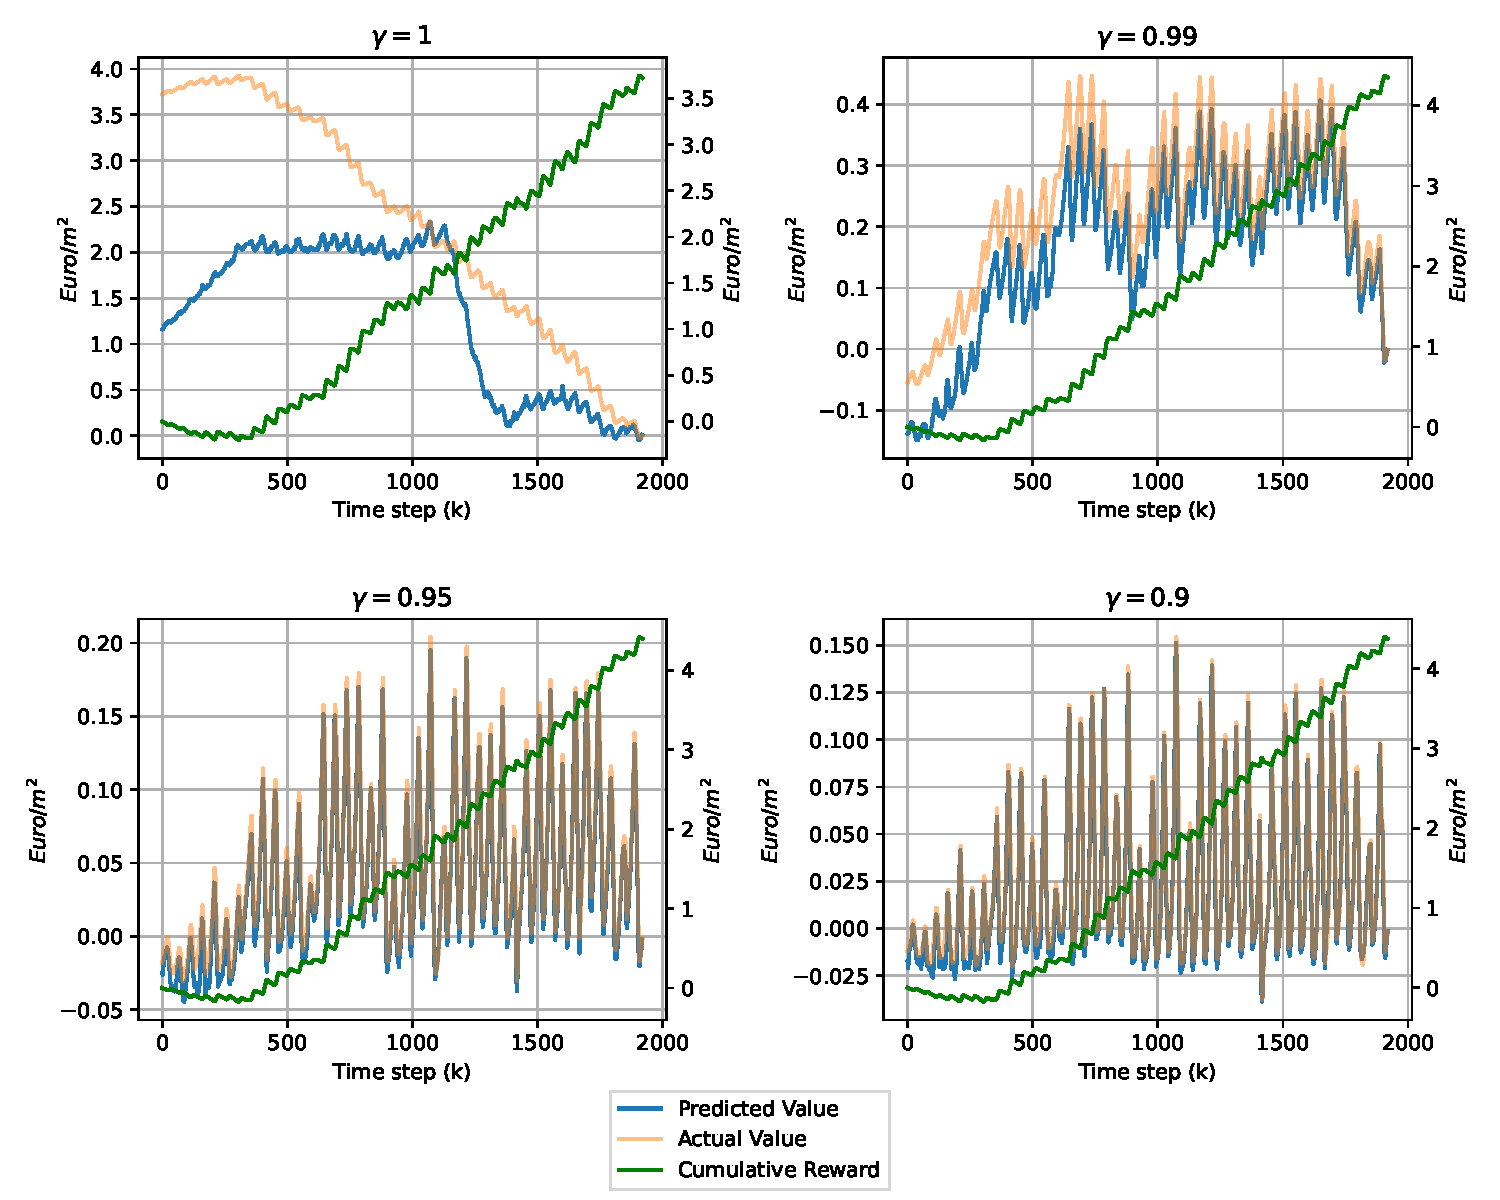
\includegraphics[width = \textwidth]{figures/vf_vs_gamma.pdf}
    \caption{Value vs Discount factor}
    \label{fig:vf-vs-gamma}
\end{figure}

The figure shown in \autoref{fig:vf-vs-gamma}  illustrates the comparison between the predicted and actual value of each state for each discount factor. In addition the cumulative reward at each time step is also logged. The left-hand side axis represents the values, while the right-hand side axis represents the cumulative reward. It is acknowledged that the trajectory of the actual value  (for $\gamma = 1$) is a horizontally reflected trajectory of the cumulative reward trajectory and can be seen in \autoref{fig:vf-vs-gamma}. Naturally this is not the case for discount factors lower than one, since the value only embeds knowledge of future rewards to be received over a shorter horizon. It is seen that the lower the discount factor, the more accurate the predicted value of a state is. This may be due to the decrease in problem complexity and therefore more accurate approximations. When $\gamma = 0.9$, the critic is capable of accurately predicting the actual value of a state. However, it falls short in accurately representing the true value of a state over the entire time horizon, given its nature of discounting future rewards. The same can be said for all discount factors lower than one. It was important to train an actor and critic with a $\gamma = 1$ because it was believed that the trained critic, despite having a worse performing policy,  could still provide a reasonable estimation of the value of a state throughout the entire simulation. Upon examining \autoref{fig:vf-vs-gamma}, it becomes evident that this assumption is incorrect. During the investigation into suitable hyper-parameters for the learning agent, it was observed that when $\gamma = 1$, the trained critic struggled to accurately estimate the value of a state in all cases. \autoref{fig:vf-vs-gamma} is just one such realization. 

\subsection{Activation Function}
It is also important for the trained critic to utilize a differentiable activation functions to ensure differentiability. This is done so that it may be used within the MPC framework. However, such an activation function, such as the commonly used tanh activation function may or may not yield desirable results in terms of maximizing cumulative reward. This section compares the performance of a learned agent with tanh activation functions against and agent with ReLu activation functions for a $\gamma = 1$ and $\gamma = 0.95$ with the ReLu acting as the baseline performance. 


\begin{table}[h!]
\centering
\begin{tabular}{|c|c|c|c|}
\hline
   & \multicolumn{2}{c|}{Performance} & \\
   \hline
  Discount Factor & ReLu & tanh & SpeedUp (\%) \\
\hline
  1   & 3.72 & 3.44 & -7.53 \\
\hline
0.95 & 4.40& 4.17& -6.08 \\
\hline
\end{tabular}
\caption{Effect of the tanh activation function}
\label{table:tanh-act-fn}
\end{table}

\autoref{table:tanh-act-fn} displays the effect of the tanh activation on the agents final performance. it is clear that ReLu significantly outperforms the tanh activation function in terms of total cumulative reward. This situation presents a dilemma. It is desirable to have an effective reinforcement learning policy in which the critic has differentiability. By incorporating the concept of differentiability into the critic, it seems that there is a decline in performance.While additional investigation into the hyperparameters may be necessary to reject this notion,  the focus of this thesis does not lie in the development of the optimal RL generated policy. Rather, \autoref{chapter:RL} aims to create a policy, and accurate critic, that is competitive with MPC so that when merged, produces a potentially better policy.

\subsection{Observation Tuples}
\todo{Might go into appendix}


\subsection{Final Results and Conclusion}
\label{section:rl-deterministic-results}
From the findings, the best policy produced by RL is with the hyperparameter shown in \autoref{tab:hyper-params}, with a $\gamma = 0.95$ and with ReLu activation functions. And while the best performing policy is desired, this configuration does not produce adequate conditions for its critic to be used in the MPC formulation, namely the value function does not hold information across the entire prediction horizon and it is not differentiable. And an agent, learned with a $\gamma = 1$ and tanh activation function results in a worse performing policy and a critic that struggles to accurately predict the value of states. With that being stated, a critic that has undergone training with a discount factor of $\gamma = 0.95$ is able to accurately predict the value of a state and may still possess sufficient knowledge regarding future rewards to be advantageous for MPC. Additionally, a critic learned with a $\gamma = 1$, albeit bad approximations, may also provide enough information. Therefore, the selected agents (the actor and the critic) to be attempted to be merged with MPC and shown in \autoref{tab:selected_agents}. 

\begin{table}[h]
    \centering
    \begin{tabular}{|c|c|c|c|}
    \hline
         Agent & $\gamma$ & Activation Function & Final Performance \\
         \hline
         Agent 1& $0.95$ & ReLu & 4.27 \\
         Agent 2& $0.95$ & Tanh & 4.18 \\
         Agent 3& $1$ & Tanh & 3.03 \\
         \hline
    \end{tabular}
    \caption{Selected Agents}
    \label{tab:selected_agents}
\end{table}

Although Agent 1, \autoref{tab:selected_agents} performs the best, its critic cannot be used in the MPC formulation. However \autoref{section:trained-vf} discusses how this issue may be addressed. 

\begin{figure}[H]
    \centering
    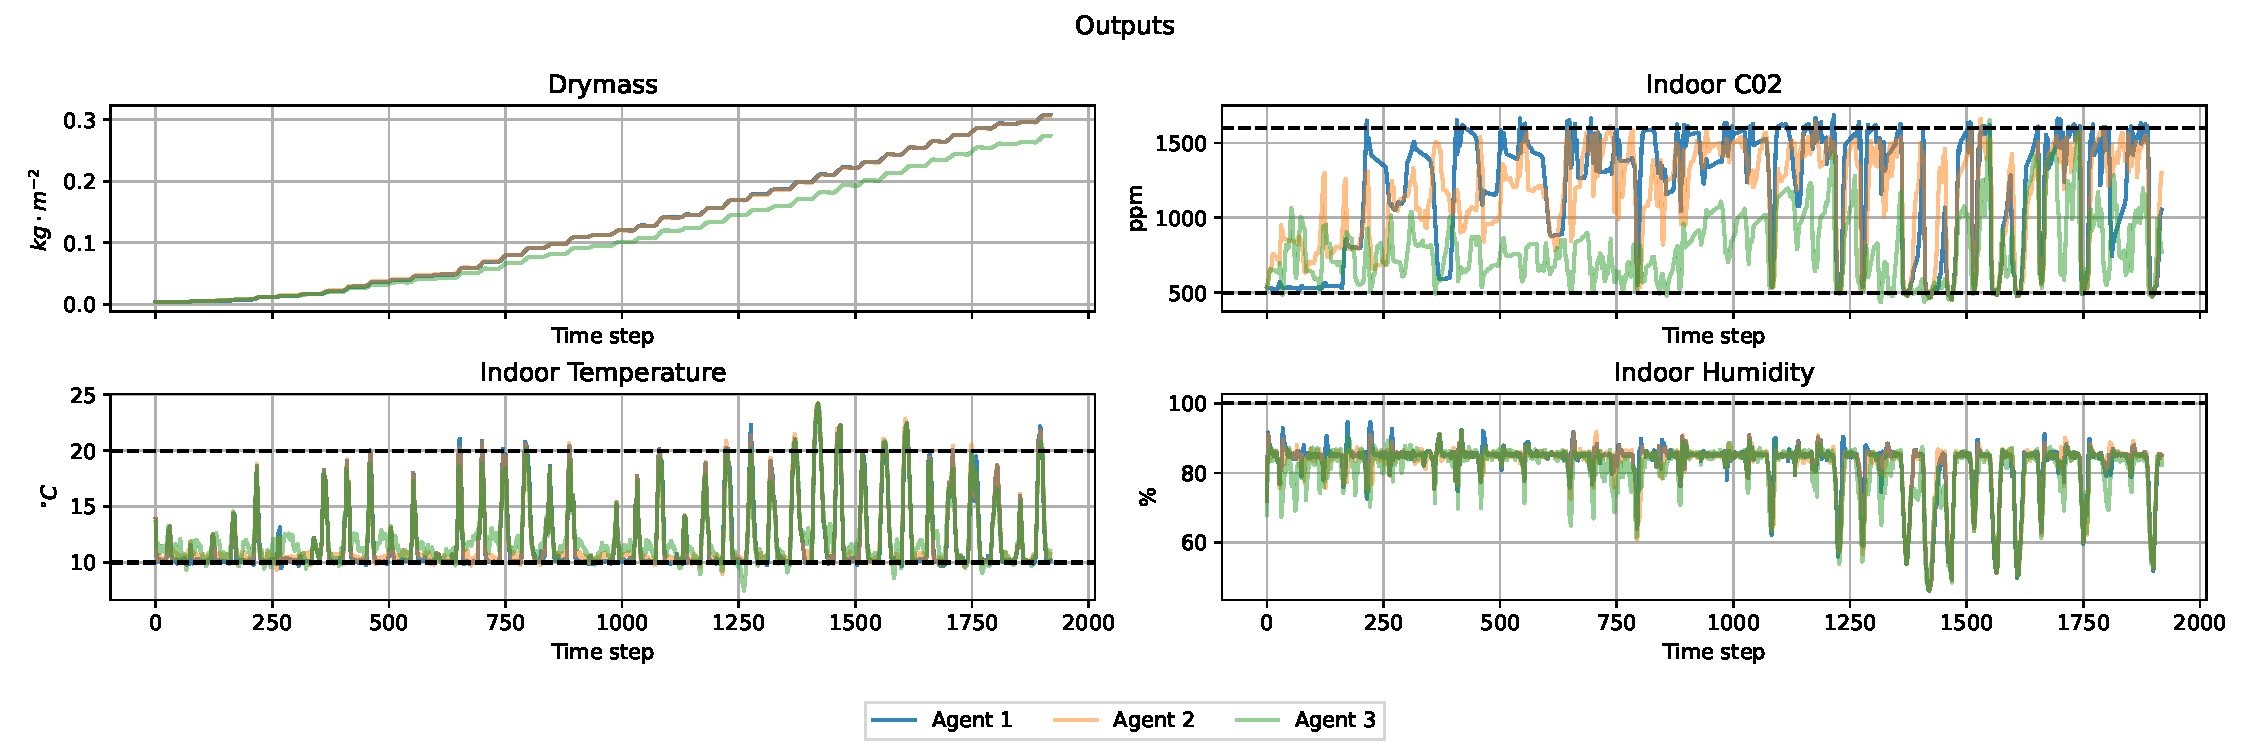
\includegraphics[width = \textwidth]{figures/selected_policies_outputs.pdf}
    \caption{Time series of system outputs}
    \label{fig:selected-policies-outputs}
\end{figure}



\begin{figure}[H]
    \centering
    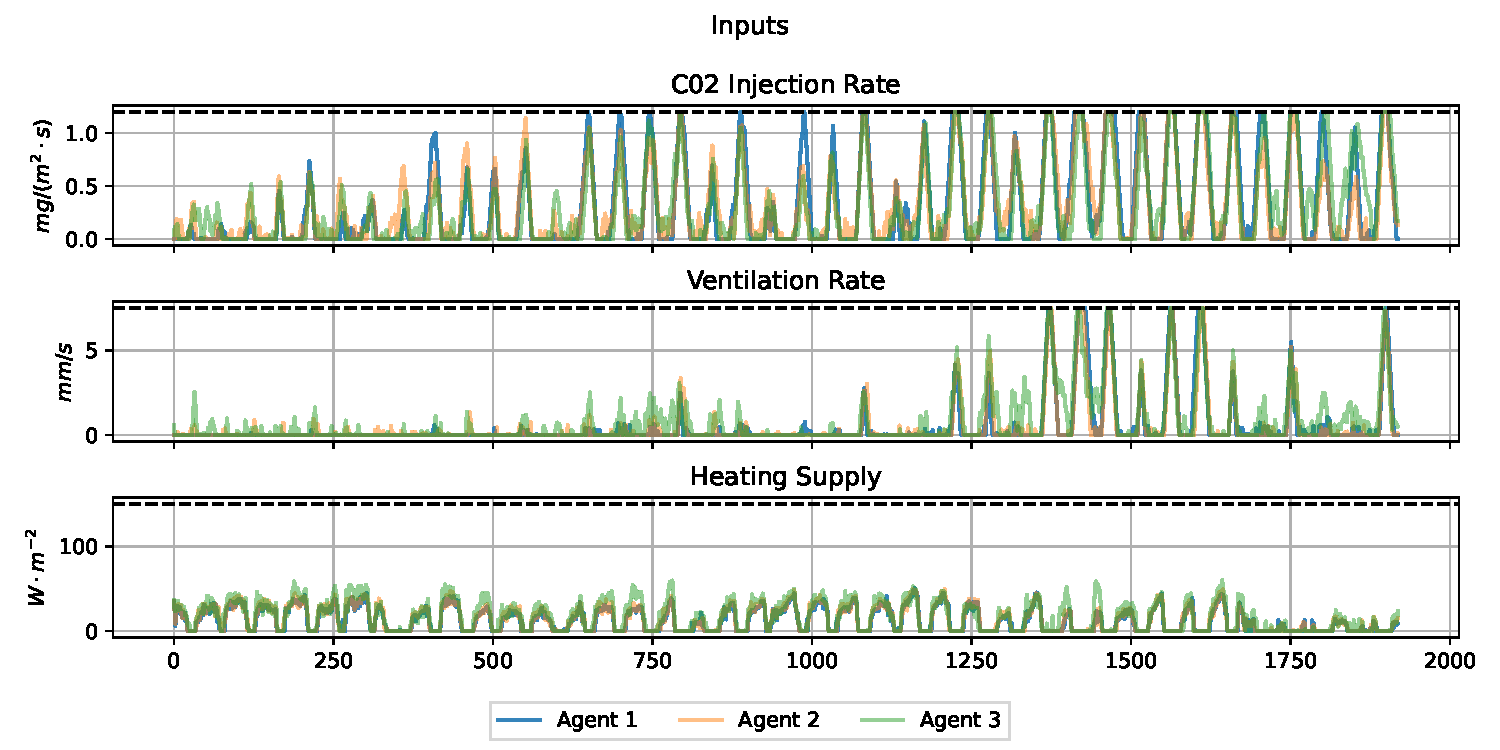
\includegraphics[width = \textwidth]{figures/selected_policies_inputs.pdf}
    \caption{Time series of system outputs}
    \label{fig:selected-policies-inputs}
\end{figure}

The time series plot of the system outputs and inputs across the 40-day period for every agent as selected in \autoref{tab:selected_agents} is shown in \autoref{fig:selected-policies-outputs}. These time series plots are similar to as those reported in \textbf{ref XXX and XXX}. Direct comparisons are not possible since in \textbf{ref XXX} does not specify the weather data range used and the reward function differs from what is used in this thesis. Furthermore, \textbf{ref XXX} include additional constraints on the temperature levels during the day to encourage heating by solar radiation during the day and the heating system by night. These constraints were not imposed in this paper as it aimed to provide RL with greater autonomy in optimizing EPI while minimizing constraint violations deemed dangerous for plant and/or human operation. Furthermore, \textbf{ref XX} also reports similar results, however a direct comparison is not possible, since hyper-parameters and reward function differs. However, it is noted that results, time series and cumulative rewards, are similar enough to give confidence in the training of the RL agent.

\begin{table}[H]
    \centering
    \begin{tabular}{|c|c|c|c|}
    \hline
         Metric& Agent 1 & Agent 2 & Agent 3  \\
         \hline
         EPI                &4.964      & 4.807     &3.727 \\
         Total Growth       &0.304      &0.303      &0.270 \\
         Total C02 Usage    &1.057      &1.0318     &1.029 \\
         Total Heating      &12.5462    &13.661     &16.381 \\
         Computational Time &0.000216   &0.00024    &0.00023 \\
         Temp Violations    &110.007    &119.2      &138.93 \\
         C02 Violations     &3311.43    &1046.47    &1972.61 \\
          Final Performance &4.27       &4.173      &3.031 \\ 
         \hline
    \end{tabular}
    \caption{Performance Metrics of agents}
    \label{tab:perf-metrics-selected-policies}
\end{table}


 Other performance metrics are reported for completeness in \autoref{tab:perf-metrics-selected-policies}. The computational time needed to compute the optimal control action is noted to take $\approx 0.2ms$. This is expected since a simple inference of the actor network is required to calculate the optimal action.
 
\section{Stochastic Results} \label{section:rl-stochastic-results}
In training the stochastic RL agent, the best hyper-parameter configuration was used, namely the same as Agent 1 (\autoref{tab:selected_agents}). Although this produces a critic that is problematic for the integration with MPC, this is solved in \autoref{section:trained-vf}. Three stochastic agents were trained, each trained on a different level of uncertainty as specified in \autoref{section:env-description} with the uncertainty model according to \autoref{eq:uncertainty_model}. All stochastic agents used the same hyper-parameters as Agent 1. Performance metrics are reported and a comparison is made with the nominal model (Agent 1 from \autoref{tab:selected_agents}). Performance metrics are evaluated by repeating the 40-day simulation period 30 times and taking the average and variance of the cumulative rewards over the complete time horizon.
Each agent is assigned a name based on the degree of uncertainty on which they received training. For example, an agent that has undergone training in a stochastic environment with a $\sigma = 20\%$ is referred to as 'Agent 0.2'. The agent named 'Agent 1' will be referred to as the 'Nominal Agent'. Each Agent is compared to the other stochastic Agents in an environment with each level of uncertainty.

\begin{figure}[H]
    \centering
    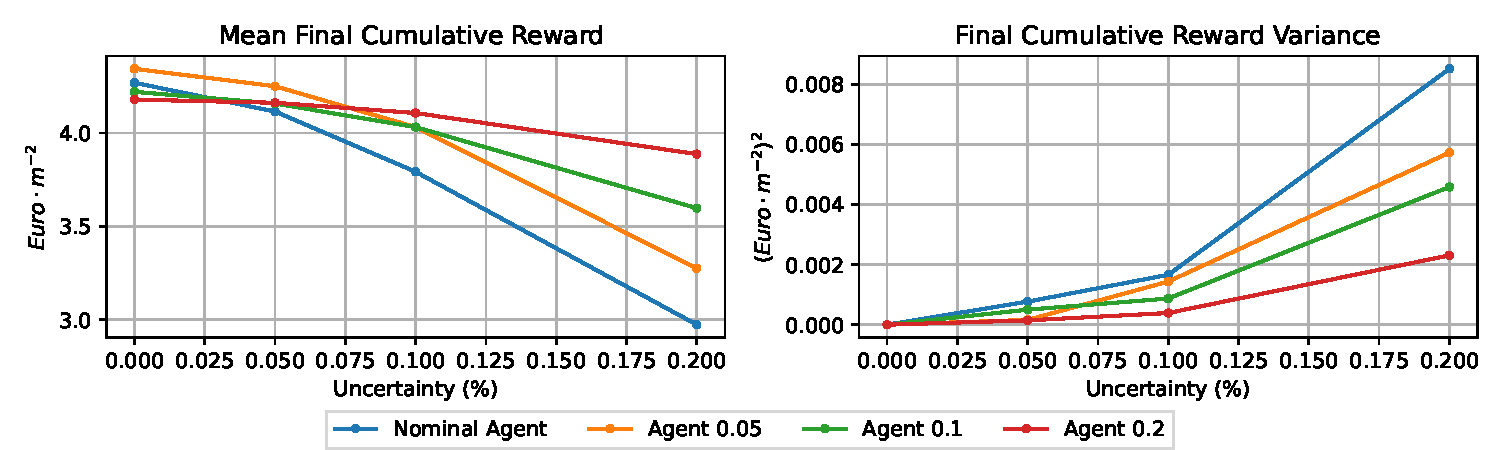
\includegraphics[width = \textwidth]{figures/stochastic_rl_policies.eps}
    \caption{Stochastic RL policy performances}
    \label{fig:stochastic-rl-policies}
\end{figure}

The final mean cumulative reward and variance of each agent under different uncertainty levels are presented in \ref{fig:stochastic-rl-policies}. As expected, as more uncertainty is injected into the environment, mean cumulative reward decreases and the variance increases. This is clear across all agents. It is also evident that each agent outperforms others in terms of performance, as indicated by higher mean cumulative reward and lower variance,  when tested on the same level of uncertainty on which it was trained. However, it seems that in the nominal case ($\sigma = 0\%$), the agent trained on a $5\%$ uncertainty level (Agent 0.05) outperforms the nominal agent, this could be due to the agent having explored more due to the noise. Moreover, Agent 0.2 seems to achieve a higher average cumulative reward than Agent 0.1 when tested on a $10\%$ uncertain model.

\subsection{Conclusion}
It is widely recognized that RL has the capability to address uncertainty through appropriate training methods, as evidenced by the findings presented in \autoref{fig:stochastic-rl-policies}. The incorporation of these stochastic policies into the MPC framework will be examined to determine whether a RL policy learned from stochastic data can transfer its characteristics to the RL-MPC framework. Finally, each agent, specifically the Nominal agent, Agent0.05, Agent0.1, and Agent0.2, is employed in its corresponding stochastic environment. Although Agent0.05 may outperform the Nominal Agent under nominal conditions, for the purpose of this thesis, its corresponding agent would be used.

\section{Trained Value Function}
\label{section:trained-vf}

Although training an agent using SAC produces an actor and a critic network, it was shown in \autoref{section:rl-deterministic-results} that the produced critic had undesirable characteristics.
This critic was trained based on a changing policy that was dependent on the critic itself, therefore it is not surprising that the approximation to the value function was sub-optimal. However this section aims at training a value function approximator with a fixed policy\footnote{This fixed policy may come from any control lay, however the RL policy is used due to its computational efficiency in determining control actions, enabling large amounts of data points and/or trajectories to be obtained}. Therefore, a value function may be trained on the best policy obtained. Additionally, there is more freedom in choosing the architecture of the value function since it is now trained independently of the policy. Therefore, simpler models may be made to approximate the value function. Specifically, upon inspection of \autoref{fig:selected-policies-outputs} and \autoref{fig:vf-vs-gamma}, it is noticed that the cumulative reward at each time step is mostly dependent on the state of the crop's dry mass at time $k$, due to the similarity in the two curves. Therefore it may be possible to learn a value approximator solely based on the crop's dry mass and current time. Two methods were employed to various value function approximators, namely the temporal difference learning method and expected return method. It is noted that this value function is only accurate under the policy it was trained on, and that the neural networks used for as the value function approximator must be made up with tanh activation functions to ensure differentiability. 



\subsection{Temporal Difference Learning}
\label{ssection:td-learning}
This method uses a similar method by which SAC, DDPG and TD3 update their critic. Most similar to DDPG. Two neural networks are used to represent the value function, a current and target network. The mean squared bellman error is minimized between the target values (from the target network) and the current values (from the current network) as shown in \textbf{eq XXX}. Moreover, a polyak averaging is used to update the target networks. 

\paragraph{Obtaining Data}
To obtain data, the nominal Agent (or Agent 1 \autoref{tab:selected_agents}) was used. A similar approach in obtaining data as in \textbf{ref xxx} was used. Along the nominal trajectory, $q$ ($q \in \mathbb{N}_{>0}$) internal states, $x$ and inputs, $u$ were uniformly sampled from $\hat{\mathbb{X}}^4$ and $\hat{\mathbb{U}}^3$ at time k respectively. So that at time $k$, a set denoted as $\hat{S}_{k} = \{\hat{s}_{k_1},\hat{s}_{k_2},...,\hat{s}_{k_q}\}$, where $\hat{s}_{k_i}$ is constructed using \autoref{eq:obs-tuple-1} from the sampled states and inputs. Each element in $\hat{S}_k$, denoted $\hat{s}_{k_i}$, is taken separately as an initial state and evolved one step in time with the RL agent, receiving a reward $\hat{r}_{k_i}$ and a boolean $d$ indicating whether a terminal state has been reached. $\hat{s}_{k_i}$ and $\hat{s}_{{k+1}_i}$ are both normalized as per \autoref{eq:agent-normalize} and stored in a transition tuple along with the received reward and $d$, denoted as $(\hat{s}_{k_i},\hat{s}_{{k+1}_i},\hat{s}_{k_i},d)$. The environment is then set back to the actual state $s_k$ and evolved for one time step, and the process repeats itself, until the 40 day period is over. The transition tuple of the actual system is also stored. To ensure a value function approximator generalizes well across the state space, the quality of sampled internal states and inputs is important. From the time series plot \autoref{fig:selected-policies-outputs} and \autoref{fig:selected-policies-inputs} is can be seen that not the entire state space needs to be sampled, especially for the dry mass state, $x_1$. The control actions were sampled across the the entire set $\mathbb{U}^3$ as shown in \textbf{eq XXX}. States $x_2,x_3,x_4$ were sampled with a range slightly larger than their respective minimum and maximum constraints range. This decision was made as it was deemed unnecessary to sample states that significantly violate constraints.  Finally, $x_1$ was sampled around the nominal $x_1$ trajectory such that the sampled state space $\hat{\mathbb{X}}^4$ is defined as:



\begin{equation}\label{eq:state_space}
\begin{split}
\hat{\mathbb{X}}^4 = \{ (x_1, x_2, x_3, x_4) \mid\ & x_1 \in [\hat{x}_{1\min}(x_{1_k}), \hat{x}_{1\max}(x_{1_k})], \\
& x_2 \in [\hat{x}_{2\min}, \hat{x}_{2\max}], \\
& x_3 \in [\hat{x}_{3\min}, \hat{x}_{3\max}], \\
& x_4 \in [\hat{x}_{4\min}, \hat{x}_{4\max}] \}
\end{split}
\end{equation}
where the bounds are specified in \autoref{tab:sample_bounds_td} and were found empirically.

\begin{table}[H]
    \centering
    \begin{tabular}{|c|c|c|}
    \hline
        Parameter& value& unit\\
        \hline
        $\hat{x}_{1\min}(x_{1_k})$ & $x_{1_k} \cdot (1-0.8) - 0.01 $ & $kg \cdot m^{-2}$\\
        $\hat{x}_{1\max}(x_{1_k})$ &$x_{1_k} \cdot (1+0.7) + 0.01 $ & $kg \cdot m^{-2}$\\
        $\hat{x}_{2\min}$ & $g_2^{-1} (\hat{x_{3_k}},400)$& $ppm$ \\
        $\hat{x}_{2\max}$ & $g_2^{-1} (\hat{x_{3_k}},1800)$& $ppm$ \\
        $\hat{x}_{3\min}$ &$7 $& $C^\circ$ \\
        $\hat{x}_{3\max}$ &$30$ &$C^\circ$\\
        $\hat{x}_{4\min}$ &$g_3^{-1} (\hat{x_{3_k}},50)$& $RH_{\%}$ \\
        $\hat{x}_{4\max}$ &$g_3^{-1} (\hat{x_{3_k}},100)$& $RH_{\%}$ \\
        \hline
    \end{tabular}
    \caption{Sample State Space bounds}
    \label{tab:sample_bounds_td}
\end{table}


\paragraph{Training}
Once data is generated, it is split into a validation and training dataset with a $20\%$ and $80\%$ split respectively to ensure that the function approximator does not over fit to the seen data. Transition tuples are sampled from the training set and the following loss function is minimized:

\begin{equation}\label{eq:vf_td_loss}
    \mathcal{L}(\phi, \mathcal{D}) =  V_{\phi}(s_k) - (r_k + (1-d) V_{\phi_{targ}} (s_{k+1}))
\end{equation}

where $\phi$ and $\phi_{targ}$ are the current and target weights of the respective function approximators and $\mathcal{D}$ is the training data set. The Adam optimizer is used to minimize \autoref{eq:vf_td_loss} over a batch size $\mathcal{B}$. The target weight $\phi_{targ}$ are updated every learning iteration by Polyak averaging $\phi$ by:

\begin{equation}
    \phi_{targ} \leftarrow (1 - \rho) \phi_{targ} + \rho \phi
\end{equation}

where $\rho$ represents the Polyak coefficient, which is a hyperparameter that needs to be tuned.


\emph{Show the sampled state space}

\subsection{Expected Return Learning}
This method includes obtaining the expected return of each state visited, from a simulated trajectory under a fixed policy, and using them as targets for that state. Compared to the temporal difference learning method, this approach has the advantage of training being significantly more stable since, in contrast to the TD method, targets remain unchanged as the function approximator's weights are updated. However, this method of learning requires a lot of data. Many trajectories must be simulated until the end, and the return must be calculated for each state visited. More importantly, only starting states are sampled, which makes it harder to obtain the same data spread as the TD-method. In contrast, the TD-method allows for higher data spread because trajectories only include one time step, which makes it possible to sample more initial states across the state space. 

\paragraph{Obtaining Data}
The same number of starting points must be sampled in order to obtain a spread that is comparable to the TD-Method; however, because the trajectory must be run through to the end of the simulation, a significantly larger amount of computational data is needed. However, targets are calculated not only for the initial state, but also for each state encountered along the trajectory. This means that fewer initial points are required, but it is still necessary to select them appropriately. A similar approach to \autoref{ssection:td-learning} was used, however, all states and inputs were uniformly sampled around a region of the nominal trajectory at time $k$ and not only the dry mass. Therefore, initial states and inputs were sampled from $\hat{\mathbb{X}^4}$ and $\hat{\mathbb{U}^3}$ and time $k$ is uniformly sampled across the entire time horizon as shown in \autoref{eq:TR-sample-space}.

\begin{equation}\label{eq:TR-sample-space}
\begin{split}
    \hat{\mathbb{X}}^4 &= \{ (\hat{x}_1, \hat{x}_2, \hat{x}_3, \hat{x}_4) \mid\ \hat{x}_1 \in [\hat{x}_{1\min}(x_{1_k}), \hat{x}_{1\max}(x_{1_k})], \\
    &\quad \hat{x}_2 \in [\hat{x}_{2\min}(x_{2_k}), \hat{x}_{2\max}(x_{2_k})], \\
    &\quad \hat{x}_3 \in [\hat{x}_{3\min}(x_{3_k}), \hat{x}_{3\max}(x_{3_k})], \\
    &\quad \hat{x}_4 \in [\hat{x}_{4\min}(x_{4_k}), \hat{x}_{4\max}(x_{4_k})] \} \\
    \hat{\mathbb{U}}^3 &= \{ (\hat{u}_1, \hat{u}_2, \hat{u}_3) \mid\ \hat{u}_1 \in [\hat{u}_{1\min}(u_{1_k}), \hat{u}_{1\max}(u_{1_k})], \\
    &\quad \hat{u}_2 \in [\hat{u}_{2\min}(u_{2_k}), \hat{u}_{2\max}(u_{2_k})], \\
    &\quad \hat{u}_3 \in [\hat{u}_{3\min}(u_{3_k}), \hat{u}_{3\max}(u_{3_k})] \} \\
    & k \sim \mathcal{U}(0,1919)  \\
\end{split}
\end{equation}

where the minimum and maximum limits are calculated as per \autoref{eq:min-max-tr-sample-space}

\begin{equation}\label{eq:min-max-tr-sample-space}
\begin{aligned}
    &\hat{z}_{min} = z_k \cdot (1-\sigma)\\
    &\hat{z}_{max} = z_k \cdot (1+\sigma)
\end{aligned}
\end{equation}

where represent the minimum and maximum range of the sample state space for a specific state, respectively, and ${z}_{k}$ represents the nominal trajectory. $\sigma$ denotes the desired spread of sampled initial states, which is expressed as a percentage.
In doing this, initial states maybe sampled around/near the nominal trajectory. As can be seen from \autoref{fig:selected-policies-inputs} and \autoref{fig:selected-policies-outputs} and later in \textbf{fig xxx}, it can be observed that the performance of policies can vary significantly with minimal changes in the nominal state and input trajectories. Therefore, this approach of sampling initial states and inputs is deemed appropriate. Finally , Agent 1 (or the nominal Agent) was used for the fixed policy. Given that the computation of a control action requires a time of $0.2 ms$, it is possible to sample a large number of trajectories in order to achieve appropriate coverage of both state and input spaces.
In the case of stochastic conditions, the same state may yield a different return, therefore if a state has been visited more than once, then the mean of the return is used as training data.

\paragraph{Training}
Once trajectories is sampled, for each state observed/visited, the total return is calculated, and the tuple $(s,TR)$ stored in a dataset. The dataset is then divided into an 80:20 ratio, with 80\% of the data used for training and 20\% used for validation.  A neural network as a function approximator is now trained with inputs as the state and labels as the total return and the loss function in \autoref{eq:vf_tr_loss} is minimized with the Adam optimizer.

\begin{equation}\label{eq:vf_tr_loss}
    \mathcal{L}(\phi, \mathcal{D}) =  \mathbb{E} [(V_{\phi}(s_k) - TR)^2]
\end{equation}

where $V_{\phi}$ is the function approximator with weights $\phi$ and $TR$ is the total return of state $s_k$. Hyper-parameters include the structure of the neural network, learning rate, and batch size.


\paragraph{Experimental Setup}
To investigate the effect of the value function in the MPC framework, it was decided to train four value functions that were based on different architects and/or states used as inputs. These models are listed in \autoref{tab:various-vf} along with their distinctive network architecture. All models were trained on 200 epochs with a learning rate of $1 \cdot 10^{-3}$ and batch size of $1024$.

\begin{table}[H]
    \centering
    \begin{tabular}{|c|c|c|c|}
    \hline
         Name & Observation Space & Hidden Layers & Neurons per layer   \\
         $V_1$& \autoref{eq:obs-tuple-1} & $2$ & $128$ \\  
         $V_2$& \autoref{eq:obs-tuple-1} & $2$ & $32$ \\  
         $V_3$& \autoref{eq:obs-tuple-1} & $1 $& $128$ \\  
         $V_4$& $(y_1(k),k)$ & $2$ & $128$ \\  
         \hline
    \end{tabular}
    \caption{Value Functions}
    \label{tab:various-vf}
\end{table}

Each value function was trained on the nominal agent, Agent 1. Additionally, $V_4$ was trained on each stochastic policy, namely 'Agent 0.05', 'Agent 0.1', and 'Agent 0.2'. 1000 trajectories were simulated and sampled from these agents, resulting in nearly one million data points consisting of states and their corresponding total return. Finally, the initial state and inputs were sampled with a spread of $\sigma = 0.5$ to ensure adequate coverage of the state and inputs spaces. The architects are chosen based on the principle that each subsequent architecture model becomes less complex, with $V_1$ serving as the initial baseline architecture. This is done to investigate the effect of these value functions in the RL-MPC framework.

Performance metrics include the squared error between the predicted total return and the actual total return as shown in \autoref{eq:vf_tr_loss}. Moreover, the accuracy of the resulting value function across the simulation period will be visualized by using \autoref{eq:v0}.

\begin{equation}\label{eq:v0}
\begin{aligned}
    V(s_k) &= r_k + V(s_{k+1}) \\
    \therefore V(s_{k-1}) &= r_{k-1} + V(s_{k}) \\
    \therefore V(s_{k-2}) &= r_{k-2} + r_{k-1} + V(s_{k}) \\
    \therefore V(s_{0}) &= \sum_{i=0}^{k-1} {r_{i}} + V(s_{k})   \\
\end{aligned}
\end{equation}

During each time step, the computation of the initial state's value will be determined by the cumulative rewards received up to that point, as well as the approximation of the current state's value using the value function. If the value function is able to approximate the value of a state accurately, then \autoref{eq:v0} should yield the same result for every time step, resulting in a horizontal line, $y = V(s_0)$.

\begin{figure}[H]
    \centering
    \includegraphics[width = \textwidth]{figures/sampled_states_TR.eps}
    \caption{Sampled States}
    \label{fig:sampled-states-TR}
\end{figure}


\begin{figure}[H]
    \centering
    \includegraphics[width = \textwidth]{figures/sampled_inputs_TR.eps}
    \caption{Sampled Inputs from Nominal conditions}
    \label{fig:sampled-inputs-TR}
\end{figure}

\autoref{fig:sampled-states-TR} and \autoref{fig:sampled-inputs-TR} are the results of all the trajectories sampled from the nominal agent. The figures reveals that the sampled trajectories exhibit a lesser extent of coverage of the state and input spaces as compared to the temporal difference learning. Nevertheless, a sufficient level of coverage is achieved. Following the completion of training and validation, a small number of additional trajectories will be sampled in order to verify the sufficient accuracy of the prediction model.


\subsection{Results}

\begin{figure}[H]
    \centering
    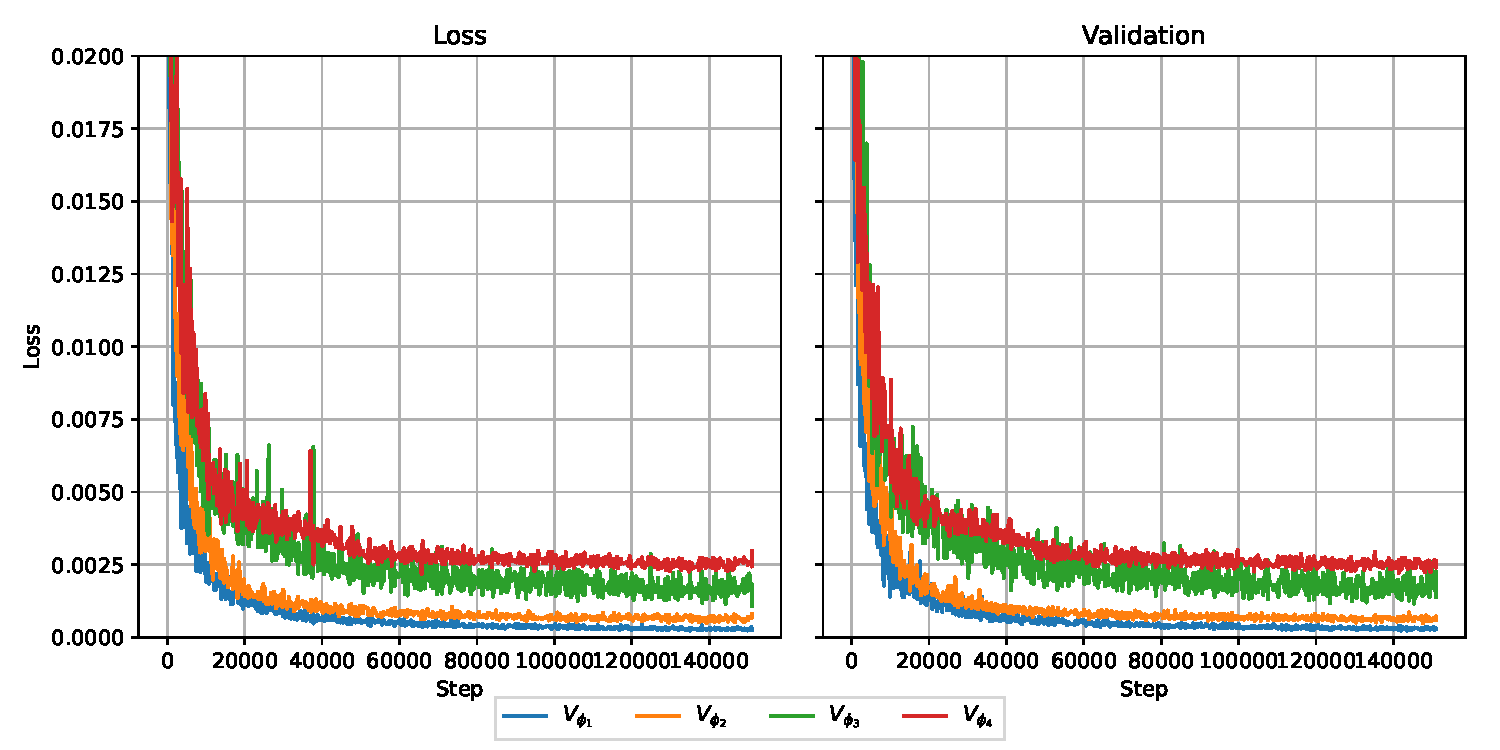
\includegraphics[width = \textwidth]{figures/tr_training_graphs.eps}
    \caption{Performance Curves, trained on the nominal Agent}
    \label{fig:tr_perf_curves}
\end{figure}


\autoref{fig:tr_perf_curves} displays the loss curves of all four models trained on data generated by the nominal agent. As expected, the baseline model ($V_1$) is able to achieve the highest accuracy compared to the simpler models.This can be attributed to its more complex structure, with each subsequent simpler model exhibiting lower accuracy. Nevertheless, when utilizing the reduced observation space model, denoted as $V_4$, the model demonstrates a high level of accuracy, as evidenced by a mean squared error of less than $0.5\%$ between the actual and predicted values.

\begin{figure}[H]
	\centering
	\begin{subfigure}[b]{0.49\textwidth}
		\centering
		\includegraphics[width=0.9\textwidth]{figures/deep_full_heatmap.eps}
		\caption{$V_1$}
		\label{fig:v1_heatmap}
	\end{subfigure}
	\hfill
	\begin{subfigure}[b]{0.49\textwidth}
		\centering
		\includegraphics[width=0.9\textwidth]{figures/deep_less_heatmap.eps}
		\caption{$V_2$}
		\label{fig:v2_heatmap}
	\end{subfigure}
	\vfill
	\begin{subfigure}[b]{0.49\textwidth}
		\centering
		\includegraphics[width=0.9\textwidth]{figures/shallow_full_heatmap.eps}
		\caption{$V_3$}
		\label{fig:v3_heatmap}
	\end{subfigure}
	\hfill
	\begin{subfigure}[b]{0.49\textwidth}
		\centering
		\includegraphics[width=0.9\textwidth]{figures/deep_reduced_heatmap.eps}
		\caption{$V_4$}
		\label{fig:v4_heatmap}
	\end{subfigure}
	\caption{Value vs Drymass vs time}
	\label{fig:vf_heatmaps}
\end{figure}


\autoref{fig:vf_heatmaps} gives a visual representation of the value of a state given the dry mass and time. It is noted that although $V_1,V_2$ and $V_3$ require an observation space as given in \autoref{eq:obs-tuple-1} to determine its value, since the value is highly dependent on the dry mass state and time, the other states in the observation space were averaged. $V_4$ naturally has an observation space of only time and the dry mass state. The lower and upper limits in \autoref{fig:vf_heatmaps} are displayed to indicate the range within which the value function approximator can be deemed reliable. This range corresponds to the portion of the sample space from which the dry mass was sampled for training. The intuitiveness of \autoref{fig:vf_heatmaps} stems from the fact that the highest return is observed at the beginning of the growing period, which can be attributed to the longer duration of the growing period. Moreover,  having a higher dry mass at any specific time leads to greater rewards, this behavior is seen across all four models within the training bounds. It is important to note that the greenhouse model limits the dry mass to a maximum of $400 g \cdot m^-2$, therefore for dry masses close to this value, very little reward can be expected, hence the lower returns in \autoref{fig:vf_heatmaps}. The primary difference is that the level of smoothness in $V_3$ as depicted in \autoref{fig:v3_heatmap} seems notably higher than that of even \autoref{fig:v4_heatmap}, which is exclusively trained on the present time and dry mass. It is anticipated that the opposite would be true, as more intricate models would be capable of fitting the data with greater precision.


\begin{figure}[H]
	\centering
	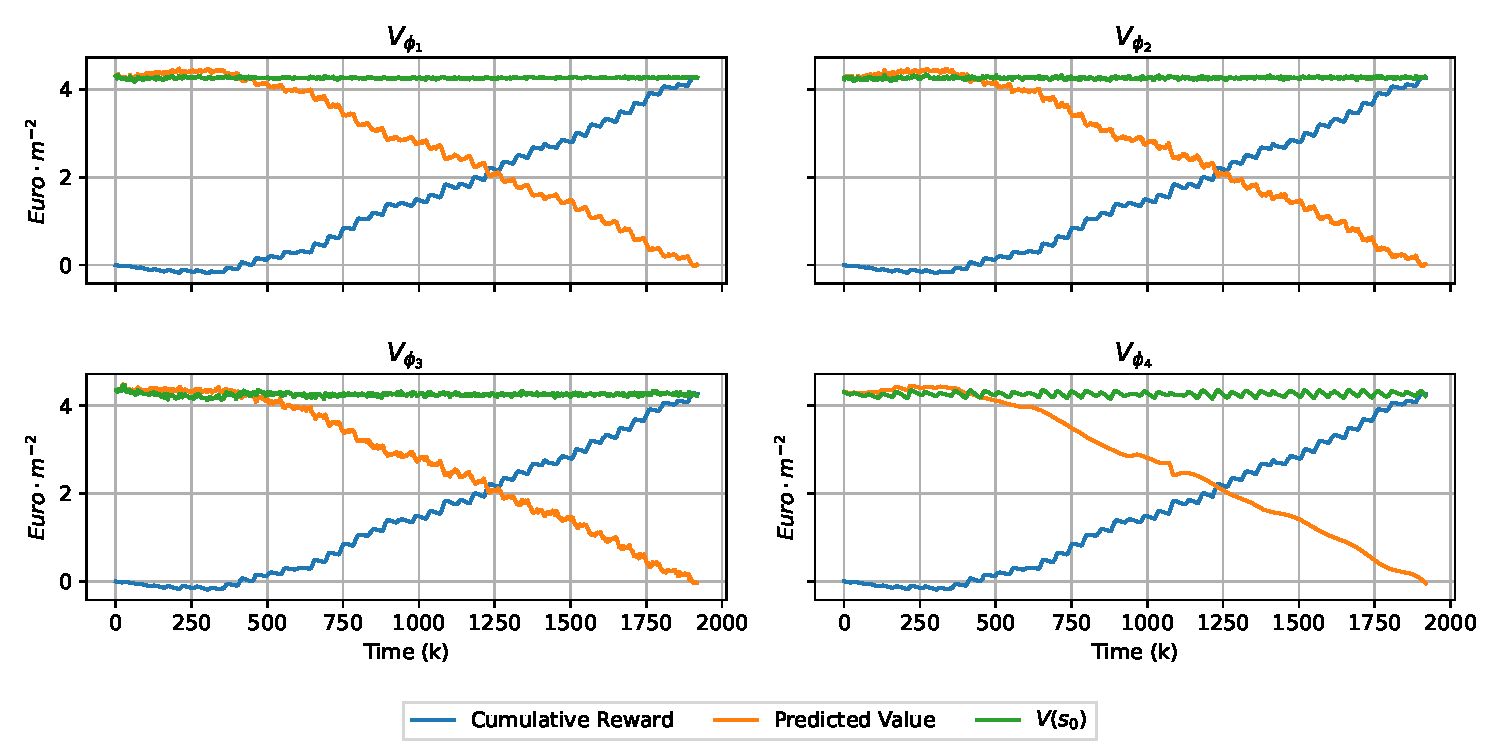
\includegraphics[width = \textwidth]{figures/vf_time_predictions_long.eps}
	\caption{Value predictions - Entire Time Horizon}
	\label{fig:tr_predictions_long}
\end{figure}

\autoref{fig:tr_predictions_long} displays a time series plot of the cumulative rewards plotted against the predicted value at each time step. This plot is similar to what is shown in \autoref{fig:vf-vs-gamma}. Additionally, it includes the calculated $V_(s_0)$ at each time step using \autoref{eq:v0} as a visual indicator of the accuracy of the value function. As demonstrated in \autoref{fig:tr_predictions_long} in conjunction with \autoref{fig:tr_perf_curves}, the predicted values show a high level of accuracy. This is evident from the nearly perfect horizontal line at $V_(s_0)$ that spans across the prediction horizon.  However, what is interesting and that cannot be seen in \autoref{fig:vf_heatmaps} is the level of noise present in each prediction. Naturally, $V_4$ is not able to make a precise prediction of the value since it only gets the time and dry mass as inputs, however its prediction is a lot smoother than all the others. This observation strongly suggests that the primary factors determining the value of a state are its drymass and time, while the minor fluctuations in rewards and corresponding expected return resulting from other factors have negligible influence across the entire time horizon.



\begin{figure}[H]
	\centering
	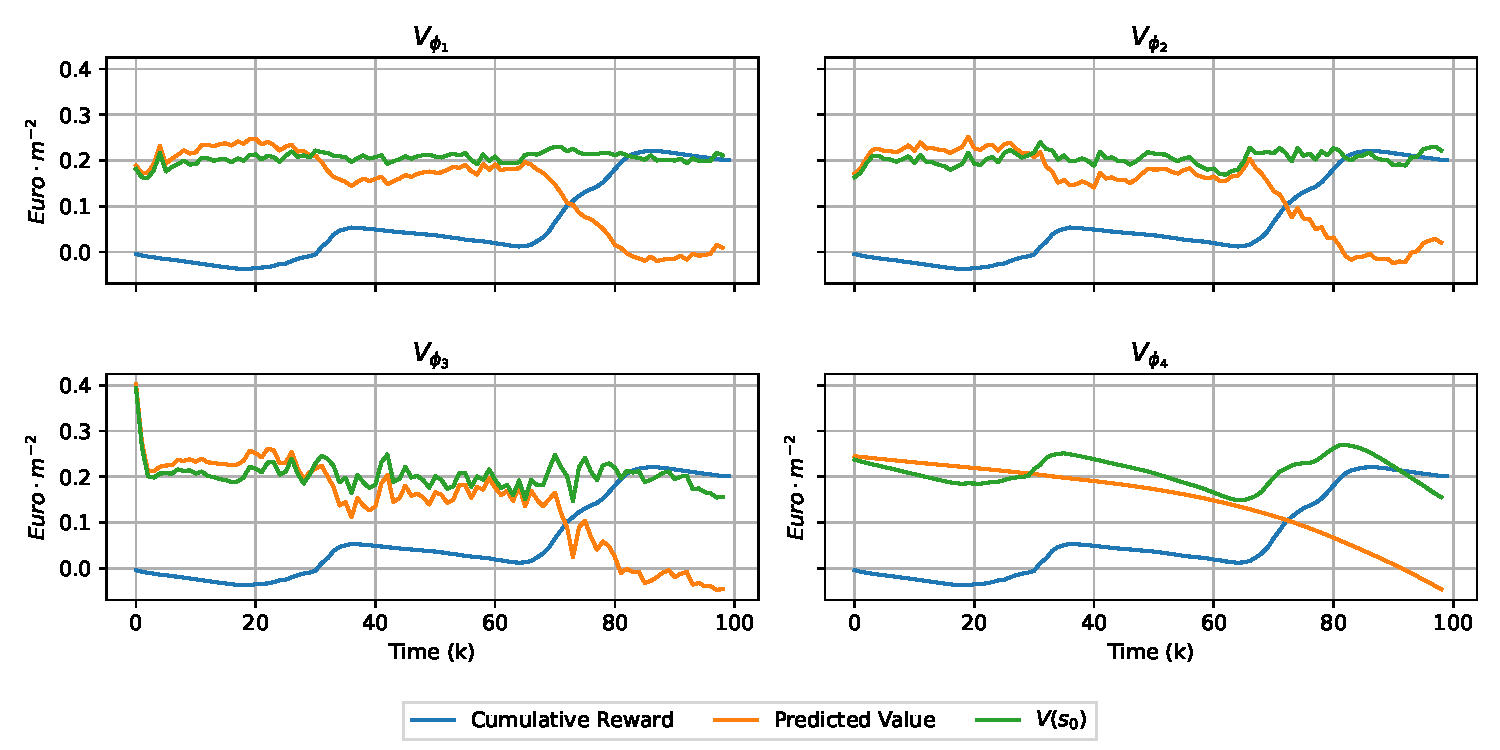
\includegraphics[width = \textwidth]{figures/vf_time_predictions_short.eps}
	\caption{Value predictions - 2 Days}
	\label{fig:tr_predictions_short}
\end{figure}

	


\autoref{fig:tr_predictions_short} shows a time series of the cumulative reward and predicted values over a two day span. 

\begin{remark}\label{rem:vf-smoothness}
	It is evident that while $V_1, V_2, V_3$ can produce more precise estimations (as demonstrated by the proximity of their prediction line $V_{s_0}$ to the actual value), $V_4$ remains significantly smoother. Moreover, $V_3$ is not as smooth as it may have seemed in \autoref{fig:vf_heatmaps} and displays the highest level of noise across the four models trained. Although this is one realization of a trajectory,this behavior was observed in all simulated trajectories.
\end{remark}



\begin{figure}[H]
	\centering
	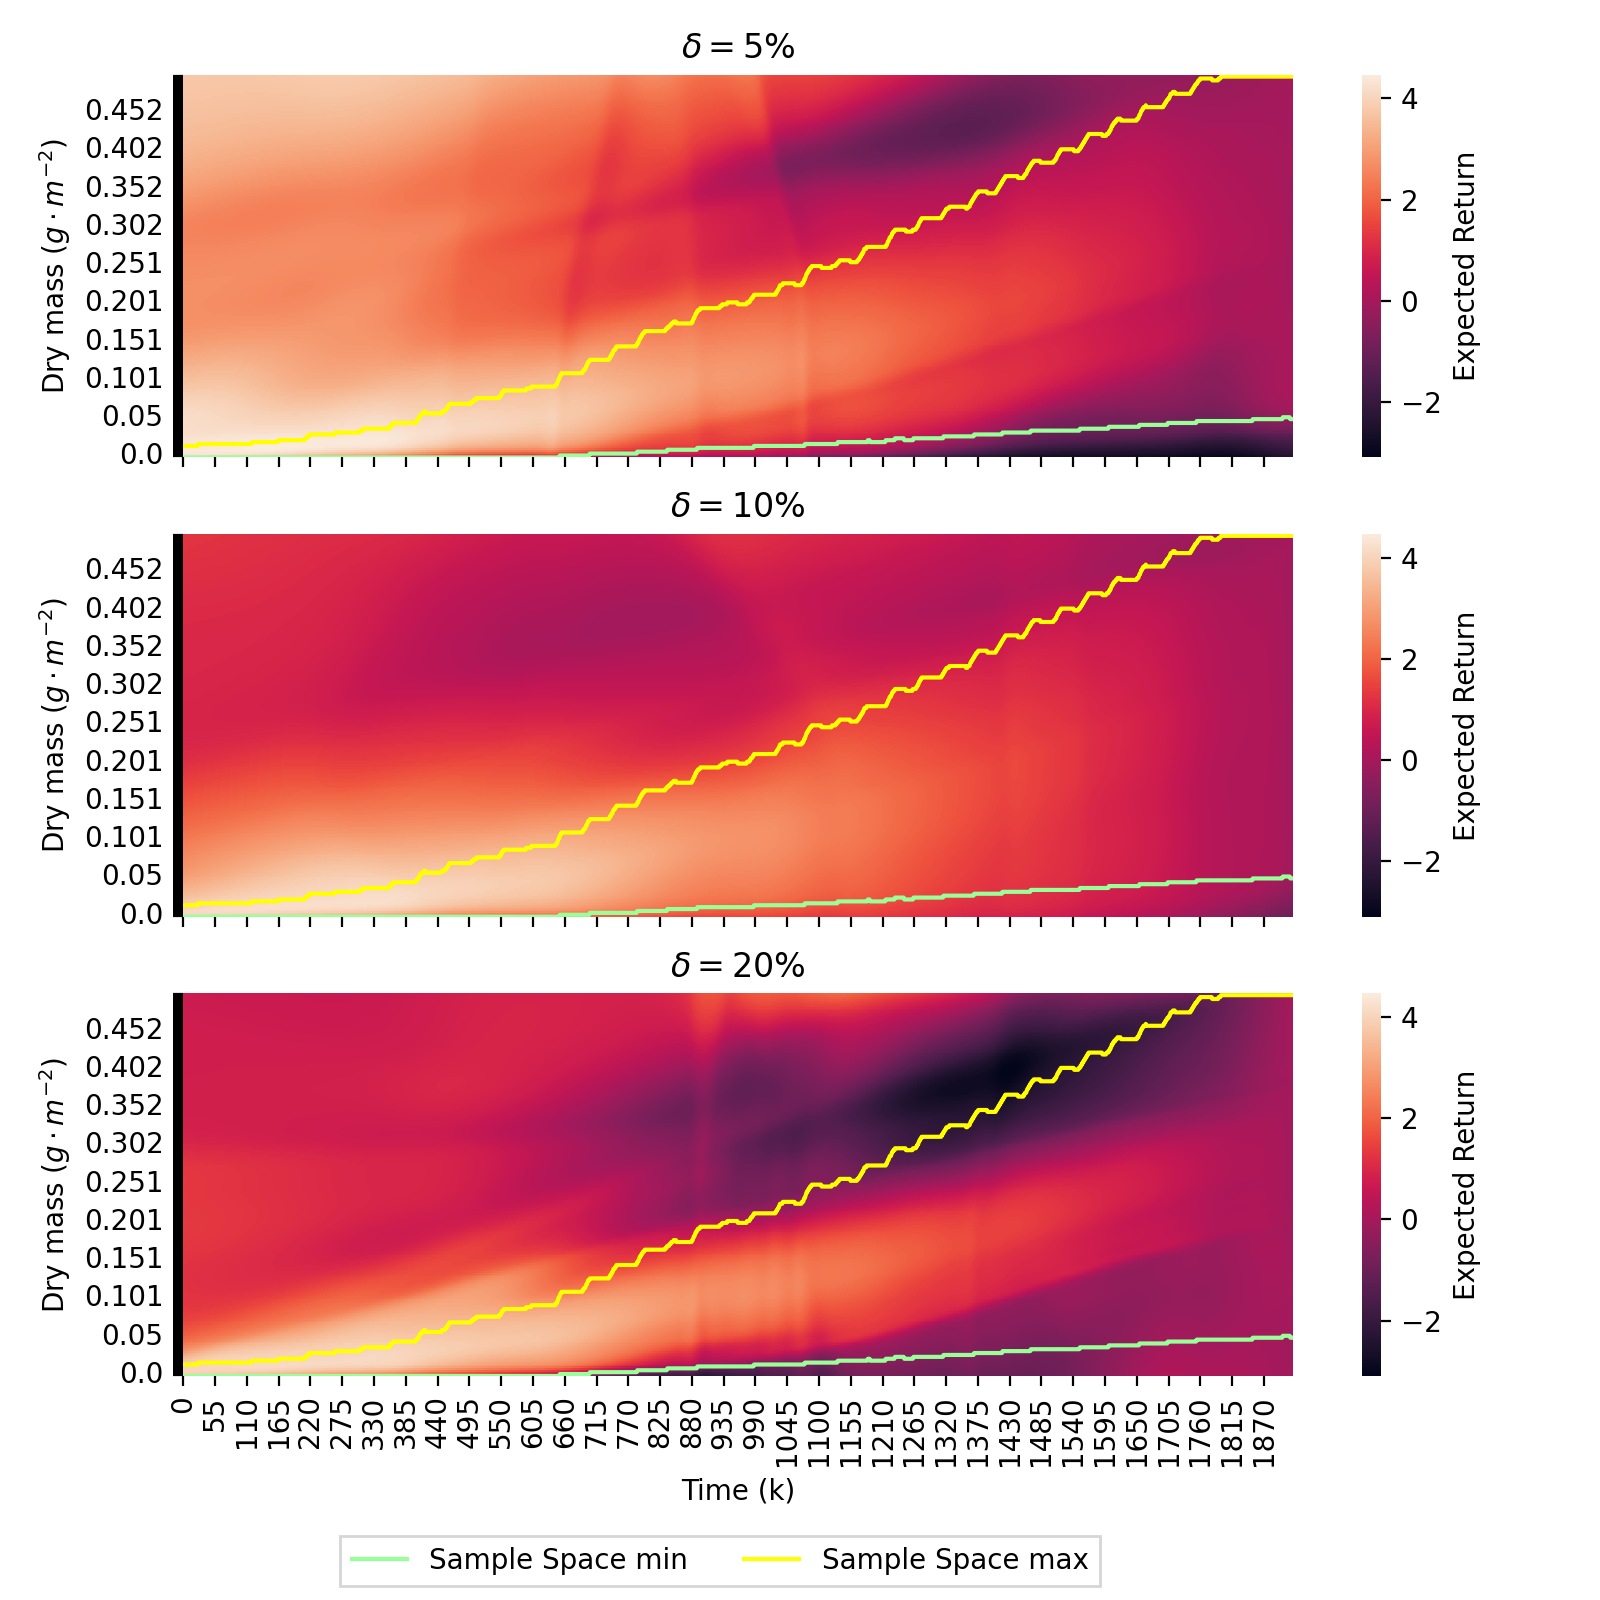
\includegraphics[width = \textwidth]{figures/vf_heatmap_stochastic.eps}
	\caption{Drymass vs Time vs Value - Stochastic}
	\label{fig:vf_heatmap_stochastic}
\end{figure}
Finally, for each level of uncertainty in the environment, a value function was trained with its corresponding agent. \autoref{fig:vf_heatmap_stochastic} displays the same heatmap as \autoref{fig:vf_heatmaps}, yielding similar behaviour as compared to the nominal conditions. However, it appears to be more coarse, particularly beyond the range of the training data.


\section{Conclusion}
The objective of this chapter was to develop a policy that is competitive with MPC and value function that can accurately approximate the expected return given the state of the environment, both for the nominal and stochastic environment. \\
It was discovered that a policy trained with a discount factor of 1 resulted in a critic that provides inaccurate value estimations and a policy that performs worse than an agent trained with lower discount factors. While reducing the discount factor leads to improved policies and a more precise critic, the critics fail to provide information about the entire growth period. Furthermore, in order to integrate the critic with MPC, it is necessary for the critic to be differentiable. This requires the use of the tanh activation function. However, using this activation function leads to a policy that is not as effective as when using a non-differentiable activation function like ReLu. \\
Given these obstacles, it became evident that additional measures were necessary. It was decided to train separate critics on the best rl policies obtained. Therefore lower discount factors and non-differentiable activation functions may be used. The best policy found and trained on the nominal data was denoted as Agent 1 with parameters shown in \autoref{tab:selected_agents}. Using the same hyper parameters as Agent 1, 3 different agents were learned based on each level of uncertainty in the greenhouse model, namely Agent0.05, Agent0.1 and Agent0.2. \\
Empirical evidence demonstrated that the stochastic agents outperformed the nominal model in terms of both the average cumulative reward and the variability in reward across different levels of uncertainty. After generating sufficient policies for both the nominal and stochastic environment, it was necessary to train an appropriate critic/value function approximator. Four different model architectures were used to train the critics, where each model architecture becomes progressively less complex. Every agent, whether in the nominal or stochastic case, had a critic that was trained to evaluate its policy under its particular level of uncertainty.\\
Results showed that accurate value function approximators could be trained, provided enough data was sampled. However, although they were accurate, the predictions were very noisy, which could be problematic later on when integrating the function appropriators into the RL-MPC framework. However, the simplest model architecture,trained on only the dry mass state and time, provided very smooth predictions, albeit not as accurate as the more complex models. It was this model architecture that was used to train value function approximators for the stochastic agents.\\
These agents and corresponding value function establishes the foundation for incorporating RL with MPC into the RL-MPC framework.
